\documentclass[11pt,a4paper]{article}
\usepackage[margin=0.85in]{geometry}
\usepackage[T1]{fontenc}
\usepackage{lmodern}
\usepackage{amsmath,amssymb,mathtools}
\usepackage{graphicx,booktabs,array,enumitem}
\usepackage[dvipsnames]{xcolor}
\usepackage{microtype}
\usepackage{caption}
\usepackage{listings}
\usepackage{hyperref}
\hypersetup{colorlinks=true,linkcolor=MidnightBlue,urlcolor=MidnightBlue,
  pdfauthor={},pdfsubject={Reinforcement learning worked solutions}}
\setlength{\parindent}{0pt}
\setlength{\parskip}{6pt}
\setlist{nosep,leftmargin=*}
\setlength{\emergencystretch}{2em}
\captionsetup{font=small,labelfont=bf}
\lstset{basicstyle=\ttfamily\small,breaklines=true,
  columns=fullflexible,keepspaces=true,showstringspaces=false,
  commentstyle=\color{gray},keywordstyle=\color{MidnightBlue},
  aboveskip=6pt,belowskip=6pt}
\newcommand{\E}{\mathbb{E}}
\newcommand{\R}{\mathbb{R}}
\newcommand{\norm}[1]{\left\lVert #1\right\rVert}
\newcommand{\sg}{\operatorname{stopgrad}}
\DeclareMathOperator*{\argmax}{arg\,max}
\DeclareMathOperator*{\argmin}{arg\,min}
\newcommand{\studytitle}[1]{%
  \hypersetup{pdftitle={#1 - Worked Solutions}}%
  {\small\color{MidnightBlue} BASICRL\quad /\quad WORKED SOLUTIONS}\par
  \vspace{5pt}{\LARGE\bfseries #1}\par\vspace{5pt}}
\newcommand{\historical}{\textbf{Experiment status.} The following numbers and
  curves are retained from earlier runs, not from a rerun of the revised
  reference code. They are examples for interpretation, not performance guarantees.\par}

\begin{document}
\studytitle{Imitation Learning: BC and DAgger}

\section{Recovery under distribution shift}
Use discounted \emph{costs}, with $0<\gamma<1$ and $0\leq\epsilon\leq1$.
Let $C$ denote cost starting safe and $D$ cost starting in the ditch. On a
safe step, a correct action costs 0; a mistake costs 1 immediately. Every
ditch action costs 1, including a successful recovery action.

\subsection{Behavior cloning}
BC never recovers after entering an unfamiliar ditch state. Thus
\begin{align*}
 D_{\rm BC}&=1+\gamma D_{\rm BC}=\frac{1}{1-\gamma},\\
 C_{\rm BC}&=(1-\epsilon)\gamma C_{\rm BC}
                  +\epsilon(1+\gamma D_{\rm BC}).
\end{align*}
Since $1+\gamma D_{\rm BC}=1/(1-\gamma)$, rearranging gives the exact answer
\[
 \boxed{J(\pi_{\rm BC})=C_{\rm BC}
 =\frac{\epsilon}{(1-\gamma)(1-\gamma+\gamma\epsilon)}.}
\]
This is at most $1/(1-\gamma)$, as expected because every step costs at most 1.

\subsection{Dataset aggregation}
DAgger's recovery succeeds with probability $1-\epsilon$. Its two equations are
\begin{align*}
 C_{\rm D}&=\gamma(1-\epsilon)C_{\rm D}
                        +\epsilon(1+\gamma D_{\rm D}),\\
 D_{\rm D}&=1+\gamma\big[(1-\epsilon)C_{\rm D}+\epsilon D_{\rm D}\big].
\end{align*}
Subtracting the first equation from the second yields $D_{\rm D}-C_{\rm D}=1-\epsilon$.
Substitution into the first equation gives
\[
 (1-\gamma)C_{\rm D}=\epsilon\big[1+\gamma(1-\epsilon)\big],
 \qquad
 \boxed{J(\pi_{\rm DAgger})
 =\frac{\epsilon(1+\gamma-\gamma\epsilon)}{1-\gamma}.}
\]

\subsection{When the familiar scaling is valid}
Writing $\delta=1-\gamma$, BC's denominator is $\delta(\delta+\gamma\epsilon)$.
The approximation $C_{\rm BC}\approx\epsilon/\delta^2$ needs
$\gamma\epsilon\ll\delta$, not merely $\epsilon\ll1$ and $\delta\ll1$.
For example, if $\epsilon=\delta$ and $\gamma\to1$, neglecting the second term
in $\delta+\gamma\epsilon$ loses a factor approaching 2.

For small $\epsilon$, DAgger has
$C_{\rm D}\approx\epsilon(1+\gamma)/(1-\gamma)$. In the regime
$\epsilon\ll1-\gamma$, BC therefore exhibits a squared effective-horizon
factor, while recovery gives DAgger a linear factor. These are properties of
this toy MDP, not universal exact formulas for all imitation-learning tasks.

\newpage
\section{Solving the cost-minimization MDP}
For a deterministic transition $s'=f(s,a)$,
\[
 Q^*(s,a)=c(s,a)+\gamma V^*(f(s,a)),\qquad
 V^*(s)=\min_a Q^*(s,a).
\]
The self-loops are mandatory and do not terminate the return. At $\gamma=0.9$,
\[
 V^*(3)=\frac{1}{1-0.9}=10,\quad
 V^*(4)=0,\quad
 V^*(5)=\frac{1.5}{1-0.9}=15.
\]
Work backward through the two decision states:
\begin{align*}
 V^*(2)&=\min\{18+0.9V^*(4),\;0+0.9V^*(5)\}
         =\min\{18,13.5\}=13.5,\\
 V^*(1)&=\min\{0+0.9V^*(2),\;2+0.9V^*(3)\}
         =\min\{12.15,11\}=11.
\end{align*}
\begin{center}
\begin{tabular}{ccl}
\toprule State & $V^*(s)$ & Optimal action\\\midrule
1 & 11 & $a_2$, move to 3\\
2 & 13.5 & $a_2$, move to 5\\
3 & 10 & $a_1$, self-loop\\
4 & 0 & $a_1$, self-loop\\
5 & 15 & $a_1$, self-loop\\\bottomrule
\end{tabular}
\end{center}
State 1 illustrates why immediate cost is insufficient: paying 2 now is
better than paying 0 and then following the more expensive continuation.

\section{Programming solution}
For continuous actions, behavior cloning minimizes the supervised loss
\[
 L_{\rm BC}(\theta)=\frac1N\sum_{i=1}^N
 \norm{\pi_\theta(o_i,g_i)-a_i^E}_2^2.
\]
Concatenate proprioception and goal along the last axis, use an MLP, and bound
the action with a hyperbolic tangent. Each training batch clears gradients,
computes predictions and MSE, backpropagates, and steps Adam. Evaluate a fixed
held-out set without gradients and select the checkpoint by validation loss.

DAgger starts from the BC dataset and repeats:
\begin{enumerate}
 \item Execute the current learner to visit its own state distribution.
 \item At each visited state, ask the expert for the target action.
 \item Add the state and \emph{expert} label to the accumulated training set.
 \item Retrain on all accumulated data and evaluate the resulting policy.
\end{enumerate}
Executing the learner while labeling with the expert is the key distinction.
Storing learner actions as targets would reinforce its mistakes. Recovery
depends on the expert being able to label the visited states and on the
learner being able to represent the needed behavior.

\newpage
\section{Reading the retained experiment}
\historical
\begin{center}
\begin{tabular}{lr}
\toprule Policy & Mean episode return\\\midrule
Random actions & $-46.2$\\
Expert & $-1.8$\\
Behavior cloning & $-11.5$\\
DAgger & $-2.3$\\\bottomrule
\end{tabular}
\end{center}
These runs use the sparse reaching reward: unsuccessful steps incur $-1$.
Less-negative returns indicate faster successful reaching under the same
evaluation convention. The random and expert rollouts used 10 episodes;
learner evaluation used 20. These small, unequal samples do not establish
a statistically reliable ranking.

\begin{figure}[h!]
 \centering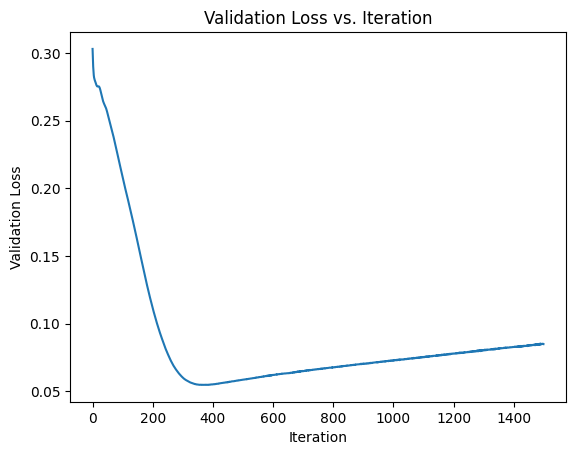
\includegraphics[width=0.82\linewidth]{figures/bc-validation.png}
 \caption{Retained BC validation curve. The late increase motivates selecting
 a validation checkpoint rather than simply using the final epoch.}
\end{figure}
The curve falls initially and later rises. That behavior is consistent with
overfitting; a low supervised loss alone also does not guarantee robust
closed-loop control outside the expert distribution. DAgger targets that
distribution mismatch by collecting labels on learner-visited states.

The revised reference uses the local shared expert checkpoint and no longer
downloads it from an external exercise repository. Its checkpoint selection
uses held-out loss. Results must be measured again after these code changes.

\textbf{Solution scope.} The exact discounted costs and MDP values follow
from the specified transitions. The empirical explanation is an interpretation
of historical observations, not a proof of an algorithm-wide performance gain.
\end{document}
